\chapter{Machine Learning}\label{machine learning}
Machine learning is a form of artificial intelligence (\ac{ai}) that involves designing and studying systems and algorithms with the ability to learn from data. This field of AI has many applications within research (such as system optimisation), products (such as image recognition) and advertising (such as adverts that use a users browsing history). There are many different paradigms that machine learning algorithms use. Algorithms can use training sets to train an algorithm to give appropriate outputs; other algorithms look for patterns in data; while others use the notion of rewards to find out if an action could be considered correct or not.~\cite{alpaydin2010introduction} Three of the most popular types of machine learning algorithms are:

\begin{itemize}
  \item \textbf{Supervised learning} is where an algorithm is trained using a training set of data. This set of data includes inputs and the known outputs for those inputs. The training set is used to fine-tune the parameters in the algorithm. The purpose of this kind of algorithm is to learn a general mapping between inputs and outputs so that the algorithm can give an accurate result for an input with an unknown output. This type of algorithm is generally used in classification systems.  
  \item \textbf{Unsupervised learning} algorithms only know about the inputs they are given. The goal of such an algorithm is to try and find patterns or structure within the input data. Such algorithm would be given inputs and any patterns that are contained would become more and more common the more inputs the algorithm is given.
  \item \textbf{Reinforcement learning} uses an intelligent agent to perform actions within an environment. Any such action will yield a reward to the agent and the agent’s goal is to learn about how the environment reacts to any given action. The agent then uses this knowledge to try and maximise its reward gains.
\end{itemize}
\section{Reinforcement Learning}\label{reinforcement learning}
In reinforcement learning an intelligent agent is learning what action to do at any given time to maximise the notion of a reward. In the beginning the agent has no knowledge of what action it should take from any state within the learning environment. It must instead learn through trial and error, exploring all possible actions and finding the ones that perform the best.

The trade-off between exploration and exploitation is one of the main features of reinforcement and can greatly affect the performance of a chosen algorithm. A reinforcement learning algorithm must contemplate this trade-off of whether to exploit an action that resulted in a large reward or to explore other actions with the possibility of receiving a greater reward.

Another main feature of reinforcement learning is that the problem in question is taken into context as a whole. This is different from other types of machine learning algorithms, as they will not considered how the results of any sub-problems may affect the problem as a whole.

The basic elements required for reinforcement learning is as follows:
\begin{itemize}
\item A Model ($M$) of the environment that consists of a set of States ($S$) and Actions ($A$).
\item A reward function ($R$).
\item A value function ($V$).
\item A policy ($P$).
\end{itemize}

The model of the environment is used to mimic the behaviour of the environment, such as predicting the next state and reward from a state and taken action. Models are generally used for planning by deciding what action to take while considering future rewards.

The reward function defines how good or bad an action is from a state. It is also used to define the immediate reward the agent can expect to receive. Generally a mapping between a state-action pair and a numerical value is used to define the reward that the agent would gain. The reward values are used to define the policy where the best value of state-action pair is used to define the action to take from a state. 

While the reward function defines the immediate reward that can be gained from a state, the value function defines how good a state will be long-term. This difference can create possible conflicts of interest for an agent; so while its goal is to collect as much reward as possible, it has to weigh up the options of picking a state that may provide a lot of up front reward but not a lot of future reward against a state with a lot of future reward but not a lot of immediate reward. This is trade-off is similar to that of exploration versus exploit as it can define how successful a reinforcement algorithm is.

The policy is a mapping between a state and the best action to be taken from that state at any given time. Policies can be simple or complex; with a simple policy consisting of a lookup table, while more complex policies can involve search processes. In general most policies begin stochastic so that the agent can start to learn what actions are more optimal.~\cite{barto1998reinforcement}

\section{Q-Learning}\label{sec:qlearning}
Q-Learning is a type of reinforcement learning algorithm where an agent tries to discover an optimal policy from its history of interactions from within an environment. What makes Q-Learning so powerful is that it will always learn the optimal policy for a problem regardless of the policy (which action a to take from a state s) it follows while learning as long as there is no limit on the number of times the agent can try an action. Due to this ability to always learn the optimal policy, Q-Learning is known as an Off-Policy learner. The history of interactions of an agent can be shown as a sequence of State-Action-Rewards:

\begin{center}
$<s_{0},a_{0},r_{1},s_{1},a_{1},r_{2},s_{2},a_{2}...>$
\end{center}

This can be described as the agent was in State 0, did Action 0, received Reward 0 and transitioned into State 1; then did Action 1, received Reward 1 and transitioned into State 2; and so on.

The history of interactions can be treated as a sequence of experiences, with each experience being a tuple.

\begin{center}
$<s,a,r,s'>$
\end{center}

The meaning of the tuple is that the agent was in State $s$, did Action $a$, received Reward $r$ and transitioned in State $s'$.  The experiences are what the agent uses to determine what the optimal action to take is at a given time.

The basic process of a Q-Learning algorithm can be seen in Figure~\ref{fig:qlearning}. The general process requires that the learning agent is given a set of states, a set of actions, a discount factor $\gamma$ and step size $\alpha$. The agent also keeps a table of Q-Values, denoted by $Q(s,a)$ where $s$ is a state and $a$ is an action from that state. A Q-Value is also an average of all the experiences the agent has with a specific state-action pair. This allows for good and bad experiences to be averaged out to give a reasonable estimation of the actual value of state-action pair. The Q-Values are defined by Equation~\ref{eq:qlearning} where $\alpha$ is the step size which specifies how much the new Q-Value is averaged with the old one, $\gamma$ is the discount factor which specifies how much the agent considers the possible future rewards it will gain and the possible future rewards ($max_{a'}Q(s',a')$) is the maximum of the Q-Values of all possible state-actions pairs from the action selected.  

\begin{equation} \label{eq:qlearning}
Q[s,a] = Q[s,a] + {\alpha}(r+ {\gamma}max_{a'} Q[s',a'] - Q[s,a])
\end{equation}

The table of Q-Values can either be initialised as empty or with some values pre-set to try and lead the agent to a specific goal state. Once the agent has initialised these parameters it observes the starting state. The starting state can either be chosen by random or be a pre-determined start state for the problem. The agent will then choose an action. Actions are chosen either stochastically or by a policy. Once an action has been chosen the agent will carry out the action and receive a reward. This reward is used to update the table of Q-Values using Equation~\ref{eq:qlearning}. Finally the agent moves into the new state and repeats until termination; which can be either when the agent discovers a goal state or after a certain number of actions have be taken.

\begin{figure}[H]
  \begin{center}
    	  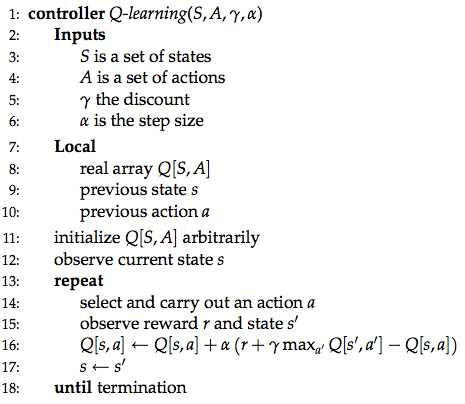
\includegraphics[width=0.5\textwidth]{figures/q-learning.jpg}
    \end{center}
    \caption{Image of Q-Learning process~\cite{poole2010artificial}.}
    \label{fig:qlearning}
\end{figure}

After a Q-Learning algorithm has finished exploring the model of the environment it creates a policy. The policy is generated by searching across all actions for a state and finding the next state with the greatest value. The policy is therefore a lookup table that maps a state with the best possible next state. The policy created can then be used to solve the problem that the Q-Learning agent was exploring.~\cite{poole2010artificial}